% Manually maintained TikZ figure for the LaTeX letter draft.
\begin{figure}[t]
\centering
\resizebox{\columnwidth}{!}{%
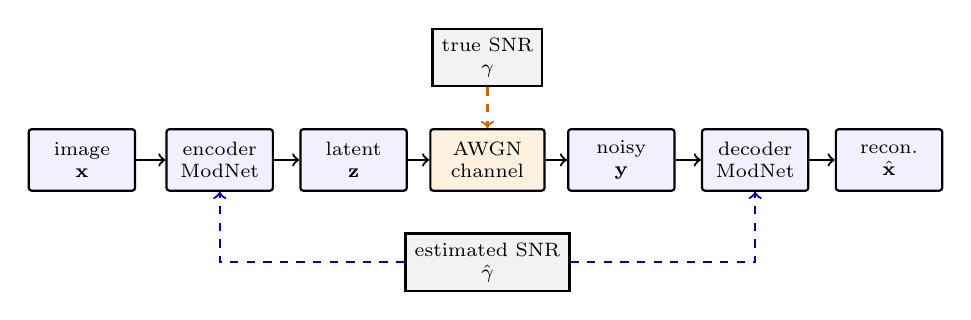
\begin{tikzpicture}[
    font=\scriptsize,
    block/.style={draw, thick, rounded corners=1pt, align=center, minimum height=0.78cm, minimum width=1.35cm, fill=blue!6},
    channel/.style={draw, thick, rounded corners=1pt, align=center, minimum height=0.78cm, minimum width=1.45cm, fill=orange!12},
    snr/.style={draw, thick, align=center, minimum height=0.5cm, minimum width=1.0cm, fill=gray!10},
    arr/.style={->, thick},
    snrarr/.style={->, thick, dashed}
]
\node[block] (x) at (0,0) {image\\$\mathbf{x}$};
\node[block] (enc) at (1.75,0) {encoder\\ModNet};
\node[block] (z) at (3.45,0) {latent\\$\mathbf{z}$};
\node[channel] (ch) at (5.15,0) {AWGN\\channel};
\node[block] (y) at (6.85,0) {noisy\\$\mathbf{y}$};
\node[block] (dec) at (8.55,0) {decoder\\ModNet};
\node[block] (xh) at (10.25,0) {recon.\\$\hat{\mathbf{x}}$};

\node[snr] (g) at (5.15,1.30) {true SNR\\$\gamma$};
\node[snr] (gh) at (5.15,-1.30) {estimated SNR\\$\hat{\gamma}$};

\draw[arr] (x) -- (enc);
\draw[arr] (enc) -- (z);
\draw[arr] (z) -- (ch);
\draw[arr] (ch) -- (y);
\draw[arr] (y) -- (dec);
\draw[arr] (dec) -- (xh);
\draw[snrarr, color=orange!80!black] (g) -- (ch);
\draw[snrarr, color=blue!70!black] (gh) -| (enc);
\draw[snrarr, color=blue!70!black] (gh) -| (dec);
\end{tikzpicture}%
}
\caption{SNR-mismatched SwinJSCC framework. The true SNR $\gamma$ determines the physical AWGN corruption, while the estimated SNR $\hat{\gamma}$ conditions the Channel ModNet branches in the encoder and decoder.}
\label{fig:framework}
\end{figure}
